\documentclass[conference]{IEEEtran}
\usepackage[utf8]{inputenc}
\usepackage[T1]{fontenc}
\usepackage[spanish,es-tabla]{babel}
\usepackage{graphicx,booktabs,amsmath,url}
\usepackage[hidelinks]{hyperref}
\title{Clasificación de radiografías de escoliosis: comparación experimental de VGG-16 y YOLO26n-cls}
\author{\IEEEauthorblockN{Yefrey Sneyder Sanchez Alba}\IEEEauthorblockA{Asignatura: Inteligencia artificial\\Universidad por completar}}
\begin{document}
\maketitle
\section*{Resumen}
Se compararon VGG-16 y YOLO26n-cls para clasificar radiografías de columna en cuatro categorías de un dataset público. El objetivo fue contrastar desempeño predictivo y costo computacional mediante un protocolo común. Tras depurar el conjunto se conservaron 5299 imágenes, distribuidas por grupos de origen en entrenamiento (3710), validación (265) y prueba (1324). Ambos modelos se ajustaron desde pesos ImageNet con cinco semillas, entradas de 224 $\times$ 224 píxeles, aumentos equivalentes y selección exclusiva por validación. Se evaluaron F1 macro, exactitud, AUROC, tiempo de ajuste, memoria y latencia en una GPU Tesla T4. VGG-16 alcanzó un F1 macro de 68,46 $\pm$ 1,07 \% y YOLO26n-cls de 65,50 $\pm$ 2,73 \%. La diferencia media fue de 2,96 puntos porcentuales a favor de VGG-16, con p = 0,0625 en una prueba exacta bilateral emparejada. YOLO redujo la latencia de 9,15 $\pm$ 0,19 a 5,35 $\pm$ 0,07 ms y presentó un menor costo de memoria. La categoría 1-derece fue la más difícil para ambos modelos. Se concluye que VGG-16 obtuvo mayor desempeño promedio observado y YOLO ofreció una alternativa de menor costo, sin evidencia estadística suficiente de superioridad al nivel de 0,05. La comparación constituye una adaptación de la referencia publicada y no una reproducción exacta de sus datos y categorías.

\textbf{Palabras clave:} escoliosis, radiografía, clasificación de imágenes, VGG-16, YOLO, aprendizaje por transferencia.

\section*{I. Introducción}
El análisis de radiografías de columna con aprendizaje profundo abarca tareas diferentes: clasificar imágenes, localizar estructuras, segmentar vértebras y medir geometría. Los resultados de esas tareas no son intercambiables. Un clasificador puede asignar una etiqueta a una imagen sin localizar una estructura ni estimar un ángulo. Por ello, la formulación del problema debe coincidir con las anotaciones y con la salida de las dos redes comparadas.

Este trabajo aborda la clasificación de cuatro etiquetas disponibles en un conjunto público. Aunque las anotaciones originales contienen cajas, cada radiografía conservada presenta una única clase distinta. Esa propiedad permite derivar un objetivo de clasificación de imagen sin inventar cajas, umbrales angulares o categorías nuevas.

\newpage
Las arquitecturas grandes pueden aprender representaciones útiles a costa de mayor memoria y tiempo de inferencia. Las variantes ligeras buscan disminuir esos costos, pero su desempeño depende del problema, de los datos y del ajuste. La comparación experimental requiere medir ambas dimensiones sobre el mismo conjunto de prueba y separar las diferencias de arquitectura de las diferencias de protocolo.

El objetivo es comparar VGG-16 y YOLO26n-cls mediante cinco ejecuciones por modelo, desempeño macro, eficiencia y análisis de errores. Se utiliza una única partición agrupada y se seleccionan checkpoints únicamente con validación. La evaluación se orienta a determinar qué ventajas observadas ofrece cada modelo bajo estas condiciones, sin atribuir utilidad clínica que no haya sido evaluada.

La contribución consiste en un experimento reproducible que integra la depuración previa, la comparación con entradas comunes, la medición de recursos y la interpretación de errores. La comparación no se limita a identificar el mayor porcentaje de aciertos: examina también la variabilidad entre semillas y la distribución del desempeño entre las cuatro categorías.

\section*{II. Trabajos relacionados}
La CNN de referencia se apoya en Baymurat et al. [1], quienes evaluaron redes preentrenadas sobre radiografías y reportaron una exactitud de 90,1 \% para VGG-16. Su estudio usa tres categorías y datos diferentes; aquí se adapta la arquitectura a cuatro salidas. Esa diferencia impide tratar sus cifras como un resultado directamente reproducido por este experimento.

Fraiwan et al. [2] utilizaron transferencia de aprendizaje para clasificar patologías de columna en radiografías. Tavana et al. [3] estudiaron tipos de curvatura mediante métodos clásicos y redes preentrenadas. Mulford et al. [4] emplearon EfficientNet-B6 para categorizar radiografías pediátricas preoperatorias y posoperatorias. Son antecedentes de clasificación, pero sus objetivos no equivalen a las cuatro etiquetas de este dataset.

Oh et al. [5] evaluaron medición automatizada de Cobb mediante CNN. Zhang et al. [6] compararon estrategias YOLOv11 y ResNet con localización y clasificación. Se distinguen de nuestro protocolo, en el que ambas redes reciben radiografías completas. VGG-16 se fundamenta en [7]; la variante clasificadora YOLO utilizada está documentada en [9].

\newpage
\section*{III. Materiales y métodos}
\subsection*{A. Datos y trazabilidad}
Se empleó el archivo del Balanced Scoliosis X-ray Dataset (YOLOv5 Format) [10] suministrado para el trabajo. Sus README declaran origen en Roboflow y licencia CC BY 4.0. La copia contiene 5960 imágenes, aunque un README anuncia una cantidad distinta. En este estudio se cuentan los archivos efectivamente disponibles y se conserva el manifiesto que relaciona cada imagen con su partición de origen.

La revisión técnica separó 619 archivos con anotaciones incompatibles para imágenes de píxeles idénticos. No se decidió automáticamente cuál de esas anotaciones era correcta. Se retiraron otras 42 copias duplicadas. Tres anotaciones poligonales se convirtieron a sus cajas envolventes y 63 cajas que excedían los bordes se recortaron a la imagen; todos los cambios quedaron registrados.

Las 5299 imágenes retenidas se agruparon transitivamente por nombre de origen anterior al sufijo de exportación, hash de archivo, hash de píxeles RGB y reflejo horizontal exacto. Una comprobación adicional con dHash de 64 bits añadió 510 enlaces de similitud: se exigió distancia Hamming $\leq$ 4 y diferencia absoluta del logaritmo de la relación de aspecto $\leq$ 0,05. Ese criterio une grupos de manera conservadora y no elimina imágenes por parecido.

El procedimiento produjo 1136 grupos. Cada grupo se asignó completo a entrenamiento, validación o prueba, aproximando 70/5/25 y equilibrando presencia de clases y cantidad de imágenes. Se verificó ausencia de cruces de las claves utilizadas. La agrupación no equivale a un identificador de paciente; se trata de una estrategia para reducir cruces de variantes conocidas.

\begin{center}\small
TABLA I. Imágenes por etiqueta original y partición.\par\medskip
\begin{tabular}{llll}
\toprule
Etiqueta & Train & Val. & Prueba\\\midrule
1-derece & 869 & 62 & 310\\
2-derece & 1015 & 73 & 362\\
3-derece & 1022 & 73 & 365\\
saglikli & 804 & 57 & 287\\
Total & 3710 & 265 & 1324\\
\bottomrule\end{tabular}\end{center}
La Tabla I cuenta imágenes, no cajas. Algunas imágenes contienen más de una caja, pero todas sus anotaciones conservadas pertenecen a la misma clase. No se fusionaron etiquetas ni se asignaron rangos de Cobb a los nombres originales. La prueba contiene 1324 imágenes pertenecientes a 317 grupos.

\newpage
\subsection*{B. Tarea y preprocesamiento}
La tarea se definió como clasificación supervisada de una radiografía en una de cuatro clases. La etiqueta se extrajo del conjunto de identificadores de clase de sus anotaciones y se verificó que ese conjunto tuviera cardinalidad uno. Las coordenadas de las cajas no se utilizaron como entrada, ni para recortar imágenes durante la evaluación.

Cada imagen se convirtió a RGB y se ajustó proporcionalmente con relleno negro hasta 224 $\times$ 224 píxeles. Esta operación conserva el encuadre completo sin imponer un recorte central. Durante entrenamiento se aplicaron reflejo horizontal con probabilidad 0,5 y rotación uniforme entre -8$^\circ$ y 8$^\circ$. Validación y prueba utilizaron el ajuste determinista, sin añadir nuevos aumentos.

Los aumentos de cada combinación imagen, época y semilla fueron generados con la misma regla para ambas redes. El orden de los lotes también se fijó por época y semilla. Esto iguala las transformaciones de entrada a una época dada, aunque las trayectorias de optimización y la duración hasta parada temprana sean distintas.

\subsection*{C. Arquitecturas y adaptación}
VGG-16 se implementó con TorchVision [12], partiendo de pesos ImageNet y sustituyendo su última capa por una salida de cuatro logits. Se ajustaron todas sus capas. Su normalización de entrada se incorporó dentro del adaptador del modelo. YOLO26n-cls partió asimismo de pesos ImageNet y se modificó su cabeza de clasificación a cuatro salidas; recibió valores de imagen en el intervalo [0,1].

La Fig. 1 resume las rutas de cálculo. Se utilizó un ciclo de entrenamiento PyTorch común, en lugar del entrenador de clasificación por defecto de Ultralytics, para mantener control sobre aumentos, presupuesto y selección. La diferencia de normalización responde a los pesos de cada modelo y se declara como parte de sus adaptadores.

\begin{center}\fbox{\parbox{.92\columnwidth}{\centering Radiografía completa\\Ajuste proporcional y relleno\\VGG-16: normalización y clasificador\\YOLO26n-cls: backbone y cabeza\\Cuatro logits por modelo}}\par\small Fig. 1. Flujos conceptuales. Esquema propio.\end{center}
La adaptación conserva la familia VGG de la referencia y algunos parámetros de ajuste, pero modifica datos, categorías, plataforma y otros detalles experimentales. El número de épocas, la paciencia, el encuadre completo y los aumentos aquí usados constituyen decisiones propias. Por tanto, el estudio reproduce una estrategia arquitectónica sobre nuevos datos, no el resultado exacto de [1].

\newpage
\subsection*{D. Entrenamiento y control experimental}
La Tabla II resume la configuración efectiva, verificada en los archivos training\_done.json de las diez ejecuciones. Se usaron cinco semillas emparejadas: 11, 22, 33, 44 y 55. La partición se mantuvo fija durante todo el experimento. Cada combinación modelo-semilla se inició en un proceso Python nuevo, con un modelo y un optimizador nuevos, evitando arrastrar estados de ejecuciones anteriores.

\begin{center}\small
TABLA II. Hiperparámetros comunes.\par\medskip
\begin{tabular}{ll}
\toprule
Parámetro & Valor\\\midrule
Entrada & 224 $\times$ 224, RGB\\
Inicialización & ImageNet; ajuste completo\\
Optimizador & SGD, momentum 0,9\\
Tasa de aprendizaje & 0,0003, constante\\
L2 / dropout & 0,004 / 0,5\\
Lote & 16\\
Pérdida & Entropía cruzada\\
Máximo / paciencia & 50 épocas / 10\\
Rotación / reflejo & $\pm$8$^\circ$ / probabilidad 0,5\\
Selección & F1 macro de validación\\
\bottomrule\end{tabular}\end{center}
Se seleccionó el checkpoint con mayor F1 macro de validación; los empates se resolvieron por menor pérdida de validación. La parada temprana se activó después de diez épocas sin mejora. No se consultó prueba para ajustar hiperparámetros o elegir un checkpoint. La evaluación final comenzó tras terminar todas las ejecuciones de entrenamiento.

Se inicializaron los generadores de aleatoriedad de Python, NumPy y PyTorch. La implementación solicitó algoritmos deterministas en modo de advertencia y desactivó TF32. Ese ajuste documenta la intención de controlar variabilidad, pero no garantiza determinismo bit a bit si una operación no dispone de una alternativa determinista. Los procesos nuevos restablecen estado de entrenamiento, sin borrar variables de entorno del sistema.

Los metadatos registran Python 3.13.16, PyTorch 2.14.1+cu130, CUDA 13.0 y GPU Tesla T4, con precisión FP32. La instalación mostrada en Colab identificó TorchVision 0.29.1+cu130 y Ultralytics 8.4.213. No se requirió entrenar desde cero: ambos modelos utilizaron transferencia de aprendizaje.

\newpage
\subsection*{E. Métricas y medición de recursos}
La métrica principal fue F1 macro: se calcula F1 en cada una de las cuatro clases y se promedian esos valores con el mismo peso. Esa decisión evita que una clase de mayor tamaño determine por sí sola el indicador. Se calcularon también exactitud, precisión macro, sensibilidad macro, especificidad uno contra el resto y AUROC macro uno contra el resto.

Para cada métrica se reporta la media y la desviación estándar muestral entre cinco semillas. La desviación estándar describe variación de entrenamiento con esta partición fija; no es un intervalo de confianza sobre pacientes. Las matrices por clase se normalizaron por fila y se promediaron entre ejecuciones. La prueba se volvió a revisar a partir de las predicciones, comprobando que coincidieran orden, etiquetas y grupos para ambos modelos.

El tiempo de ajuste incluye entrenamiento y validación, con guardado de checkpoints; excluye descarga inicial de pesos y prueba. Se midieron parámetros entrenables y memoria GPU máxima asignada por PyTorch. La memoria no representa la totalidad reservada por el controlador o por otros procesos, por lo que se reporta con su definición operacional.

La latencia corresponde a la red y su adaptador en FP32, con lote uno y una entrada precargada en GPU. Se ejecutaron 20 calentamientos y 100 repeticiones con sincronización antes y después de cada medición. Se excluyen lectura, transformación y transferencia de imágenes. Las cifras caracterizan este escenario, no la demora total de una aplicación clínica.

\subsection*{F. Comparación estadística}
Se aplicó una prueba exacta bilateral de permutación emparejada [11]. La estadística fue la media de las diferencias de F1 macro, definidas como YOLO menos VGG en cada semilla. Se enumeraron los 32 intercambios posibles dentro de los cinco pares. La hipótesis nula supone intercambiabilidad de resultados entre modelos dentro de cada par, equivalente a simetría de signos de las diferencias.

El nivel de referencia se fijó en $\alpha$ = 0,05. Con cinco pares, la resolución mínima bilateral es 2/32 = 0,0625. Por ello, esta prueba no puede alcanzar un valor menor que 0,05 con el diseño usado, incluso cuando los cinco pares favorecen a una red. Se informa el resultado y el tamaño observado de la diferencia, sin presentar ausencia de significación como equivalencia.

\newpage
\section*{IV. Resultados}
\subsection*{A. Desempeño global}
Las diez ejecuciones terminaron y se evaluaron sobre las mismas 1324 imágenes. La reconstrucción independiente de sus matrices de confusión reprodujo el F1 macro de los archivos de métricas. La Tabla III resume los indicadores predictivos. VGG-16 obtuvo los valores medios más altos en este conjunto; YOLO26n-cls presentó mayor variabilidad entre semillas para F1 y exactitud.

\begin{center}\small
TABLA III. Desempeño en prueba: media $\pm$ DE, cinco semillas.\par\medskip
\begin{tabular}{lll}
\toprule
Métrica & VGG-16 & YOLO26n-cls\\\midrule
Exactitud (\%) & 69,62 $\pm$ 0,98 & 65,85 $\pm$ 2,55\\
Precisión macro (\%) & 69,50 $\pm$ 1,23 & 66,16 $\pm$ 2,89\\
Sensibilidad macro (\%) & 69,34 $\pm$ 1,20 & 65,68 $\pm$ 2,52\\
F1 macro (\%) & 68,46 $\pm$ 1,07 & 65,50 $\pm$ 2,73\\
Especificidad macro (\%) & 89,81 $\pm$ 0,34 & 88,57 $\pm$ 0,84\\
AUROC macro & 0,905 $\pm$ 0,006 & 0,884 $\pm$ 0,010\\
\bottomrule\end{tabular}\end{center}
La diferencia media de F1 fue de 2,96 puntos porcentuales a favor de VGG-16. La Tabla IV muestra que esa dirección se mantuvo en las cinco semillas, aunque la magnitud varió de 0,36 a 7,22 puntos. El resultado no se reduce, por tanto, a una sola ejecución excepcional de VGG, pero tampoco describe una ganancia constante.

\begin{center}\small
TABLA IV. F1 macro por semilla y diferencia en puntos porcentuales.\par\medskip
\begin{tabular}{llll}
\toprule
Semilla & VGG (\%) & YOLO (\%) & YOLO-VGG\\\midrule
11 & 69,57 & 62,35 & -7,22\\
22 & 67,64 & 65,50 & -2,14\\
33 & 67,24 & 63,24 & -3,99\\
44 & 69,53 & 68,45 & -1,08\\
55 & 68,33 & 67,97 & -0,36\\
\bottomrule\end{tabular}\end{center}
La enumeración de permutaciones reprodujo p = 0,0625. No se rechaza la hipótesis nula al nivel de 0,05. Este resultado debe leerse con la resolución del diseño: es el menor valor bilateral alcanzable con cinco pares y no invalida la diferencia descriptiva observada. La inferencia se refiere a semillas sobre una partición fija, no a una población independiente de pacientes.

\newpage
\subsection*{B. Eficiencia y costo computacional}
La Tabla V muestra la contraparte computacional. YOLO26n-cls redujo la latencia media un 41,56 \%, equivalente a una razón VGG/YOLO de aproximadamente 1,71. También utilizó menos parámetros y menor memoria máxima asignada. Estas diferencias corresponden a las implementaciones adaptadas a cuatro clases, no a los modelos originales con sus cabezas ImageNet.

\begin{center}\small
TABLA V. Recursos en Tesla T4, FP32. Tiempo: media $\pm$ DE.\par\medskip
\begin{tabular}{lll}
\toprule
Medida & VGG-16 & YOLO26n-cls\\\midrule
Ajuste (min) & 23,42 $\pm$ 5,90 & 17,35 $\pm$ 2,49\\
Latencia (ms) & 9,15 $\pm$ 0,19 & 5,35 $\pm$ 0,07\\
Parámetros (millones) & 134,28 & 1,54\\
Memoria asignada (MiB) & 3092,86 & 328,94\\
Épocas finales (rango) & 14-26 & 18-25\\
\bottomrule\end{tabular}\end{center}
El modelo VGG adaptado tiene 134276932 parámetros frente a 1536228 de YOLO, una razón de aproximadamente 87,41. La razón de memoria asignada fue 9,40. El tiempo medio de ajuste de YOLO fue un 25,93 \% menor, aunque las épocas finales difirieron por parada temprana. Igualar el presupuesto máximo no implica igual número de actualizaciones efectivamente ejecutadas.

\begin{center}
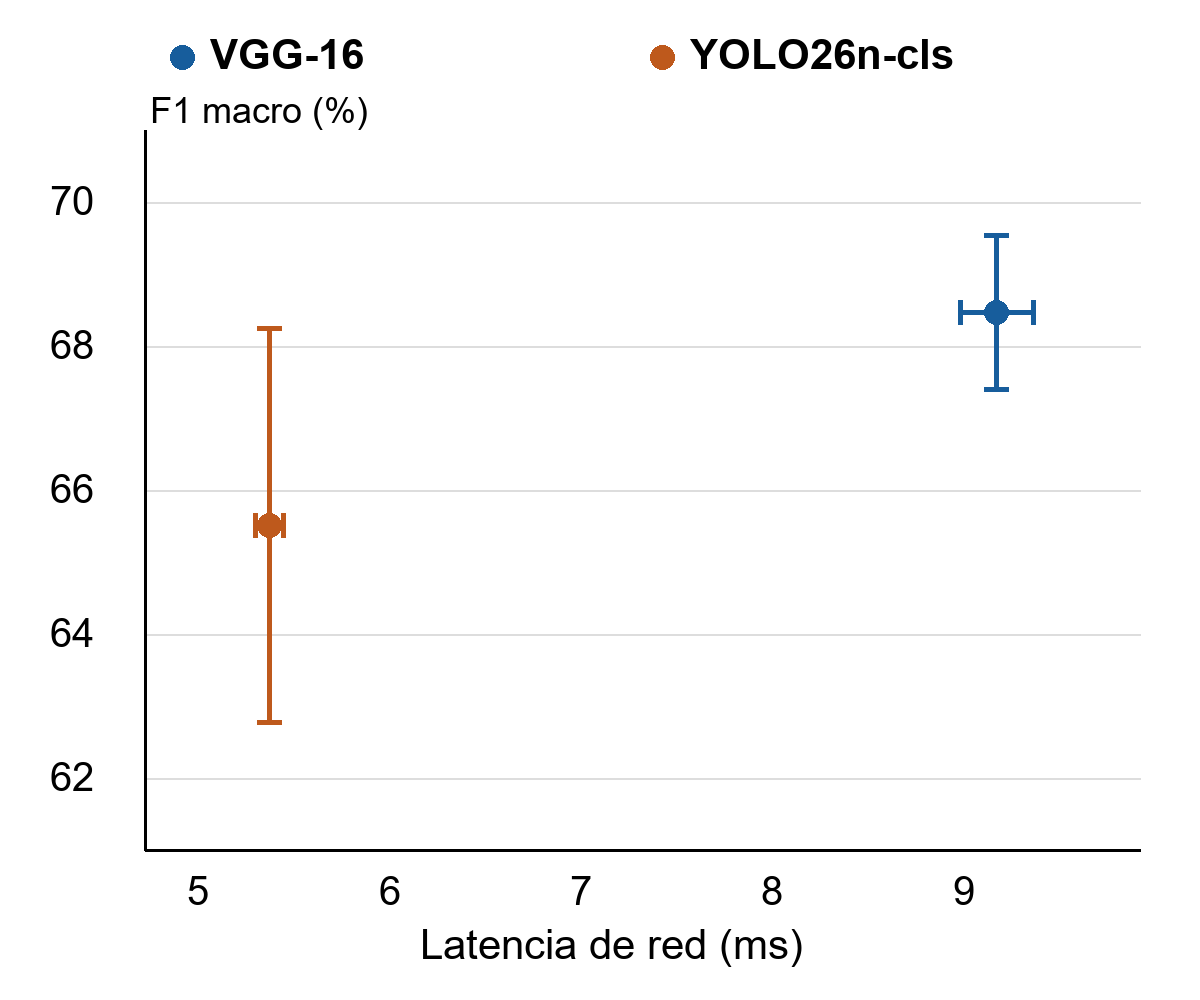
\includegraphics[width=\columnwidth]{figures/desempeno_latencia.png}
\par\small Fig. 2. F1 macro de prueba frente a latencia media de red. Las barras muestran DE entre semillas, no intervalos de confianza poblacionales.
\end{center}
La Fig. 2 expresa el compromiso de esta comparación: VGG está situado en mayor F1 y mayor latencia, mientras YOLO ocupa la región de menor latencia y menor F1 promedio. No hay un modelo que domine simultáneamente ambas medidas. La elección depende del peso asignado a desempeño y recursos, sin extrapolar estas mediciones a otros tamaños de entrada o hardware.

\newpage
\subsection*{C. Aprendizaje y selección de checkpoints}
\begin{center}
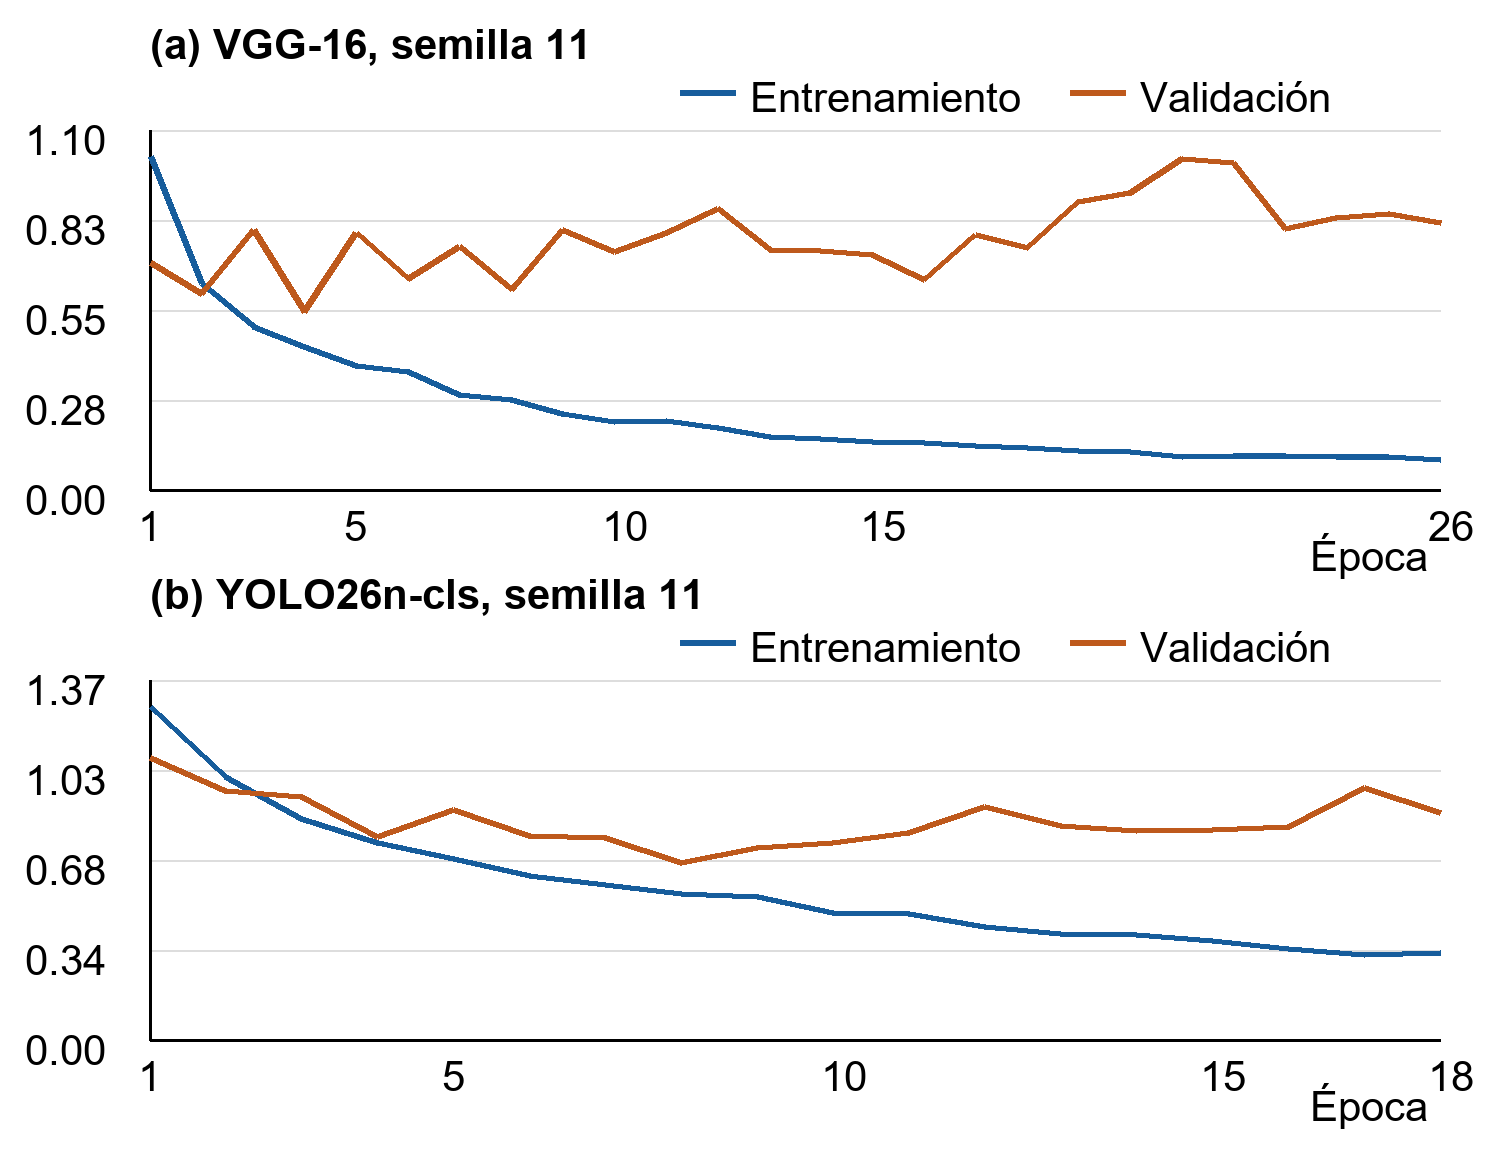
\includegraphics[width=\columnwidth]{figures/curvas_semilla11.png}
\par\small Fig. 3. Pérdidas de entrenamiento y validación de la semilla 11, fijada de antemano. (a) VGG-16. (b) YOLO26n-cls. Las curvas no promedian ejecuciones con duraciones distintas.
\end{center}
La Fig. 3 muestra una disminución de la pérdida de entrenamiento en ambas redes y una separación posterior respecto a validación. En la semilla 11, VGG finalizó con pérdidas de entrenamiento y validación de 0,093 y 0,820; YOLO, de 0,334 y 0,865. Esa separación es compatible con sobreajuste y justifica utilizar un checkpoint anterior seleccionado por validación, sin asumir que la última época sea la mejor.

En VGG, los checkpoints seleccionados correspondieron a las épocas 16, 4, 15, 11 y 7. En YOLO fueron 8, 15, 11, 15 y 10, en el mismo orden de semillas. Todas las ejecuciones se detuvieron antes de alcanzar 50 épocas. No se escogió la mejor semilla por prueba: las cinco se conservaron en el resumen.

El mayor F1 de validación de VGG osciló entre 0,771 y 0,809; el de YOLO, entre 0,644 y 0,710. La comparación final utiliza prueba y no esas cifras. La validación contiene 265 imágenes en 65 grupos, lo cual proporciona menos diversidad que la prueba y puede introducir variabilidad en la selección del checkpoint.

\newpage
\subsection*{D. Errores por categoría}
\begin{center}
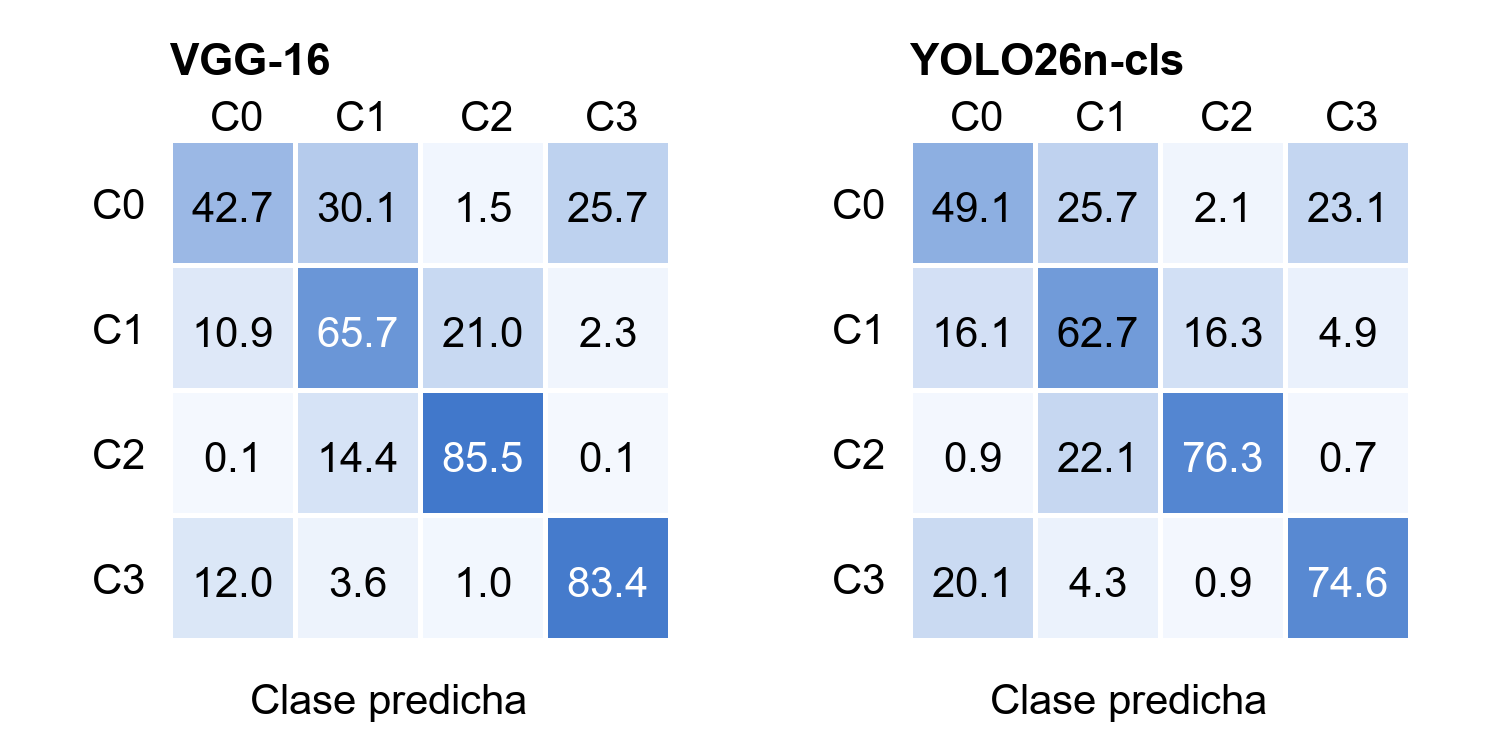
\includegraphics[width=\columnwidth]{figures/confusiones_medias.png}
\par\small Fig. 4. Matrices de confusión medias normalizadas por fila. Cada celda es un porcentaje; las cinco evaluaciones reutilizan las mismas imágenes y no representan 6620 casos independientes. C0, C1, C2 y C3 siguen el orden de etiquetas de la Tabla I.
\end{center}
\begin{center}\small
TABLA VI. Sensibilidad media por clase (\%).\par\medskip
\begin{tabular}{lll}
\toprule
Etiqueta & VGG-16 & YOLO26n-cls\\\midrule
1-derece & 42,71 & 49,10\\
2-derece & 65,75 & 62,65\\
3-derece & 85,48 & 76,33\\
saglikli & 83,41 & 74,63\\
\bottomrule\end{tabular}\end{center}
La Tabla VI y la Fig. 4 identifican 1-derece como la clase de menor sensibilidad para ambos modelos. VGG asignó, en promedio, el 30,06 \% de esa clase a 2-derece y el 25,74 \% a saglikli. En YOLO, esas proporciones fueron 25,68 \% y 23,10 \%. El desempeño global no describe por sí solo esa dificultad específica.

YOLO obtuvo mayor sensibilidad en 1-derece, a pesar de su menor F1 macro total. VGG presentó mayor sensibilidad en las otras tres clases. En consecuencia, no es correcto afirmar que VGG sea mejor en todas las categorías. La inspección por clase aporta información que se pierde al comparar únicamente los promedios.

En 3-derece, YOLO confundió el 22,08 \% con 2-derece, frente al 14,41 \% de VGG. La principal confusión de saglikli fue hacia 1-derece: 20,14 \% en YOLO y 11,99 \% en VGG. Se reportan los nombres originales; no se interpreta esa proximidad nominal como una escala clínica validada ni se atribuyen causas médicas a cada error.

El análisis identifica patrones de clasificación, pero no adjudica etiquetas correctas alternativas. Las diferencias de encuadre, contraste o fondo deben verificarse mediante revisión sistemática; estos resultados por sí solos no permiten establecer que una de esas propiedades causó las equivocaciones.

\newpage
\subsection*{E. Interpretación visual con Grad-CAM}
Se generaron mapas Grad-CAM [8] para VGG-16 en la primera semilla prefijada, usando seis errores y dos aciertos en orden de archivo. La Fig. 5 presenta dos errores y dos aciertos de esa selección. Los mapas se calcularon para la clase predicha sobre la última salida espacial del extractor, por lo que ofrecen una localización gruesa y no una segmentación anatómica.

\begin{center}
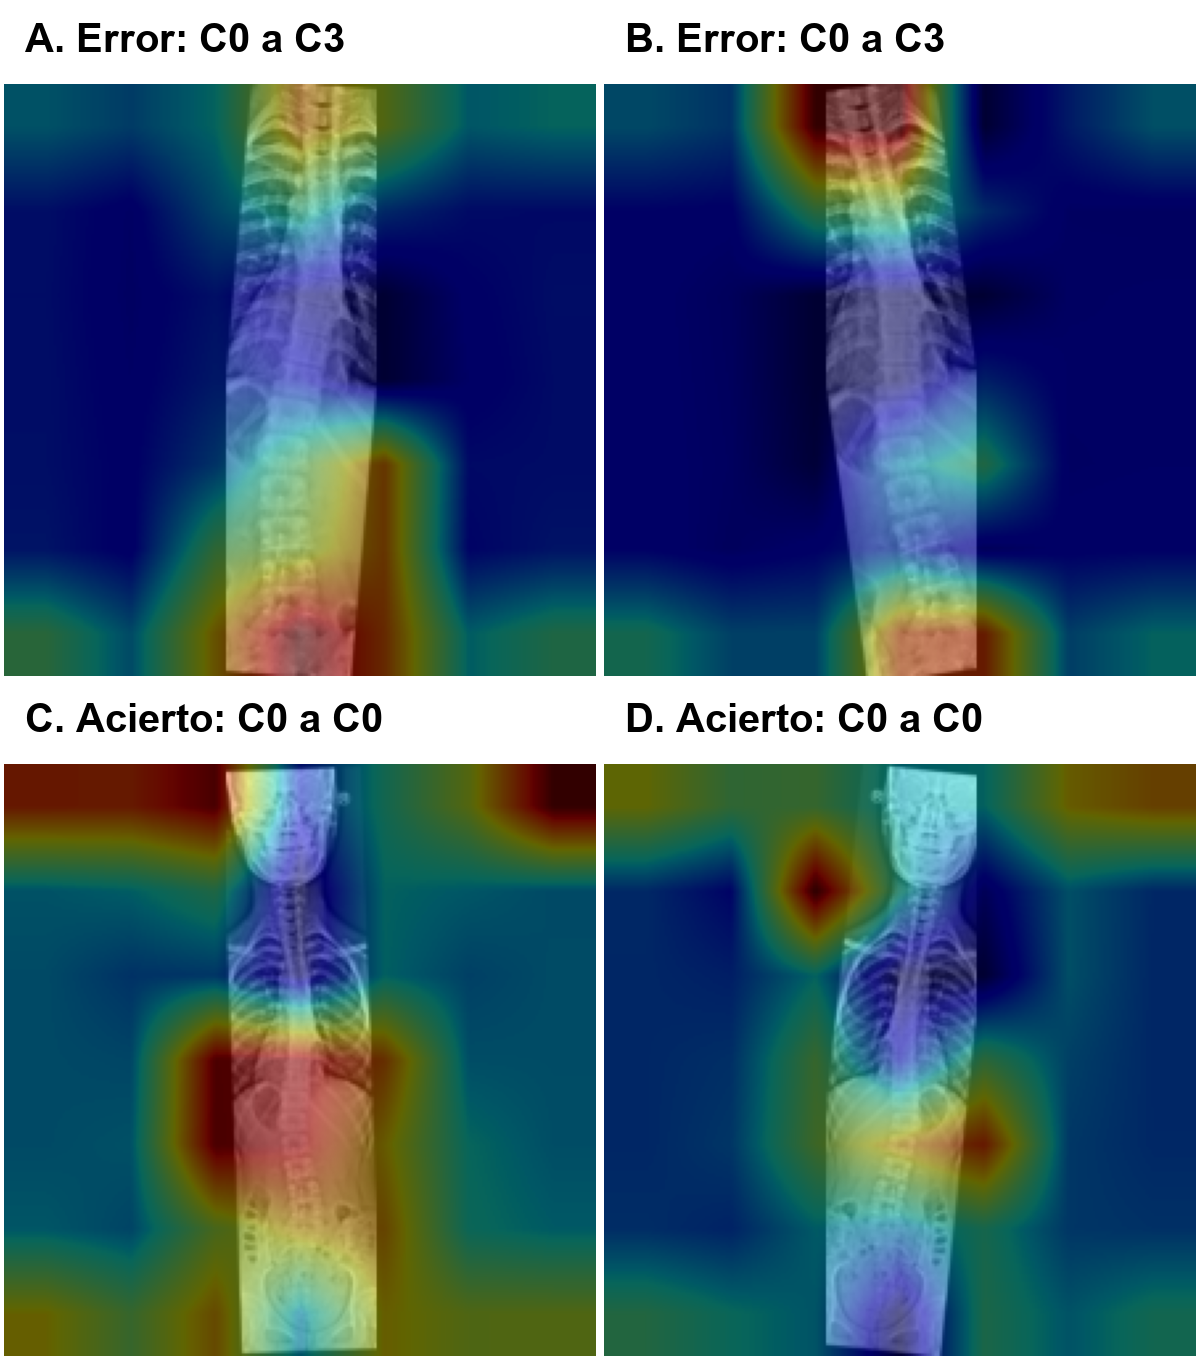
\includegraphics[width=\columnwidth]{figures/gradcam_ejemplos.png}
\par\small Fig. 5. Grad-CAM de VGG-16, semilla 11. A-B: errores. C-D: aciertos. C0 = 1-derece; C3 = saglikli. Los códigos indican clase real y predicha, en ese orden. Los colores cálidos indican mayor activación relativa dentro de cada mapa.
\end{center}
Las activaciones no se restringen visualmente al eje de la columna. En los ejemplos se observan regiones cálidas sobre áreas anatómicas y sobre bordes o relleno de fondo. Esa extensión sugiere examinar dependencia del encuadre y del contexto, pero la resolución del mapa y su interpolación impiden afirmar que el fondo determine causalmente la decisión.

Un mapa en un acierto tampoco demuestra razonamiento clínico correcto. La técnica describe sensibilidad de la salida a características internas, no ofrece una explicación causal ni verifica la validez de las etiquetas. Por ello, los ejemplos acompañan las métricas y se presentan como análisis exploratorio.

\subsection*{Disponibilidad y uso de IA}
Código, manifiesto y CSV se incluyen en el paquete reproducible. Repositorio: https://github.com/Sneyderx/comparacion-escoliosis-vgg16-yolo. El enlace de Colab puede añadirse como complemento de ejecución. Se utilizó asistencia de IA para apoyar preparación del código, análisis y redacción; el autor debe revisar el contenido y las referencias antes de entregar.

\newpage
\section*{V. Discusión}
El resultado central es un compromiso entre desempeño y costo. VGG-16 logró mayor F1 promedio y menor dispersión entre semillas. YOLO26n-cls redujo latencia, tiempo de ajuste y memoria. La categoría 1-derece mostró una excepción al orden global: su sensibilidad fue mayor con YOLO. Estas observaciones favorecen una recomendación condicionada al escenario, en lugar de declarar un ganador universal.

Las dos AUROC macro fueron superiores a 0,88, mientras F1 y exactitud fueron menores. No existe contradicción: AUROC evalúa ordenación de puntuaciones uno contra el resto, mientras la clasificación final selecciona la mayor puntuación entre cuatro categorías. Una buena ordenación no garantiza una frontera multiclase bien resuelta. No se ajustaron umbrales ni calibración usando prueba.

La comparación con el resultado publicado de la referencia requiere cautela: cambian datos, clases, encuadre y plataforma. La distancia numérica entre porcentajes no estima un efecto arquitectónico aislado. La evidencia presentada permite evaluar una adaptación sobre este dataset, sin acreditar que se reprodujo exactamente el experimento original.

La prueba exacta no alcanzó significación a 0,05 porque el diseño de cinco pares tiene una resolución mínima de 0,0625. Las cinco diferencias favorecieron a VGG, pero el tamaño muestral experimental es pequeño. Las repeticiones cuantifican variabilidad de entrenamiento; no sustituyen nuevas cohortes ni cinco particiones independientes.

Como limitaciones, se dispone de una sola partición, no hay identificadores de paciente verificados y permanecen aumentos preexistentes. La depuración reduce cruces detectados, sin garantizar independencia por paciente. La comparación comparte hiperparámetros en lugar de optimizar cada red por separado; por ello describe el protocolo común y no la mejor configuración posible de cada arquitectura.

\section*{VI. Conclusiones}
En las condiciones evaluadas, VGG-16 obtuvo F1 macro de 68,46 \% frente a 65,50 \% de YOLO26n-cls, sin evidencia estadística suficiente de superioridad a $\alpha$ = 0,05. YOLO mostró menor latencia y costo de memoria. Para priorizar F1 global en este experimento, VGG es la opción con mejor media observada; para priorizar recursos, YOLO ofrece una alternativa más ligera, aceptando la pérdida de desempeño medida.

Como trabajo futuro se propone evaluar originales sin aumentos con partición por paciente, ampliar repeticiones mediante un diseño fijado previamente y contrastar configuraciones específicas de cada red. Los errores de 1-derece y la sensibilidad al contexto merecen revisión antes de considerar cualquier uso fuera del ejercicio académico.

\newpage
\section*{Referencias}
[1] A. C. Baymurat et al., “Scoliosis screening from plain radiographs including chest and abdominal X rays by using the deep learning method: Is it worth?,” J. Turk. Spinal Surg., vol. 35, no. 2, pp. 49-54, 2024. DOI: 10.4274/jtss.galenos.2024.41736. \url{https://doi.org/10.4274/jtss.galenos.2024.41736}
\par\medskip
[2] M. Fraiwan, Z. Audat, L. Fraiwan y T. Manasreh, “Using deep transfer learning to detect scoliosis and spondylolisthesis from x-ray images,” PLOS ONE, vol. 17, no. 5, e0267851, 2022. DOI: 10.1371/journal.pone.0267851. \url{https://doi.org/10.1371/journal.pone.0267851}
\par\medskip
[3] P. Tavana, M. Akraminia, A. Koochari y A. Bagherifard, “Classification of spinal curvature types using radiography images: Deep learning versus classical methods,” Artif. Intell. Rev., vol. 56, pp. 13259-13291, 2023. DOI: 10.1007/s10462-023-10480-w. \url{https://doi.org/10.1007/s10462-023-10480-w}
\par\medskip
[4] K. L. Mulford et al., “Deep learning classification of pediatric spinal radiographs for use in large scale imaging registries,” Spine Deform., vol. 12, no. 6, pp. 1607-1614, 2024. DOI: 10.1007/s43390-024-00933-9. \url{https://doi.org/10.1007/s43390-024-00933-9}
\par\medskip
[5] H. Y. Oh, T. K. Kim, Y. S. Choi, M. Park, R. G. Yoon y J. K. An, “Radiographic analysis of scoliosis using convolutional neural network in clinical practice,” J. Korean Soc. Radiol., vol. 85, no. 5, pp. 926-936, 2024. DOI: 10.3348/jksr.2023.0111. \url{https://doi.org/10.3348/jksr.2023.0111}
\par\medskip
[6] H. Zhang, J. Qi y Z. Zhang, “Spinal x-ray based scoliosis diagnosis using deep learning: A comparison of YOLOv11 and ResNet,” Biomed. Eng. / Biomed. Tech., vol. 71, no. 4-5, pp. 519-535, 2026. DOI: 10.1515/bmt-2026-0192. \url{https://doi.org/10.1515/bmt-2026-0192}
\par\medskip
[7] K. Simonyan y A. Zisserman, “Very deep convolutional networks for large-scale image recognition,” en ICLR, 2015. arXiv:1409.1556. \url{https://arxiv.org/abs/1409.1556}
\par\medskip
[8] R. R. Selvaraju et al., “Grad-CAM: Visual explanations from deep networks via gradient-based localization,” en ICCV, 2017. Texto de la publicación original. \url{https://openaccess.thecvf.com/content_ICCV_2017/papers/Selvaraju_Grad-CAM_Visual_Explanations_ICCV_2017_paper.pdf}
\par\medskip
[9] Ultralytics, “Image classification with Ultralytics YOLO,” documentación técnica. Consultado: 14 nov. 2026. docs.ultralytics.com/tasks/classify/. \url{https://docs.ultralytics.com/tasks/classify/}
\par\medskip
[10] salmankey, “Balanced Scoliosis X-ray Dataset (YOLOv5 Format),” Kaggle. Consultado: 14 nov. 2026. Página del conjunto de datos. La copia suministrada declara CC BY 4.0 y origen Roboflow en sus README. \url{https://www.kaggle.com/datasets/salmankey/balanced-scoliosis-x-ray-dataset-yolov5-format}
\par\medskip
[11] SciPy, “scipy.stats.permutation\_test,” documentación técnica. Consultado: 14 nov. 2026. Referencia de permutation\_test. \url{https://docs.scipy.org/doc/scipy/reference/generated/scipy.stats.permutation_test.html}
\par\medskip
[12] TorchVision, “vgg16,” documentación técnica. Consultado: 14 nov. 2026. Referencia de vgg16 y pesos preentrenados. \url{https://docs.pytorch.org/vision/stable/models/generated/torchvision.models.vgg16.html}
\par\medskip
\end{document}